\documentclass[../main.tex]{subfiles}
% 2.2.1 Was ist es?
Das klassische Doppelspaltexperiment weist das Wellenartige Verhalten von Licht durch die Interferenz der Wellen nach.
% 2.2.2 Geschichte / Entdeckung
Das Experiment wurde erstmals 1801 von Thomas Young durchgeführt \cite{TODO}.

\begin{figure}[ht]
    \centering
    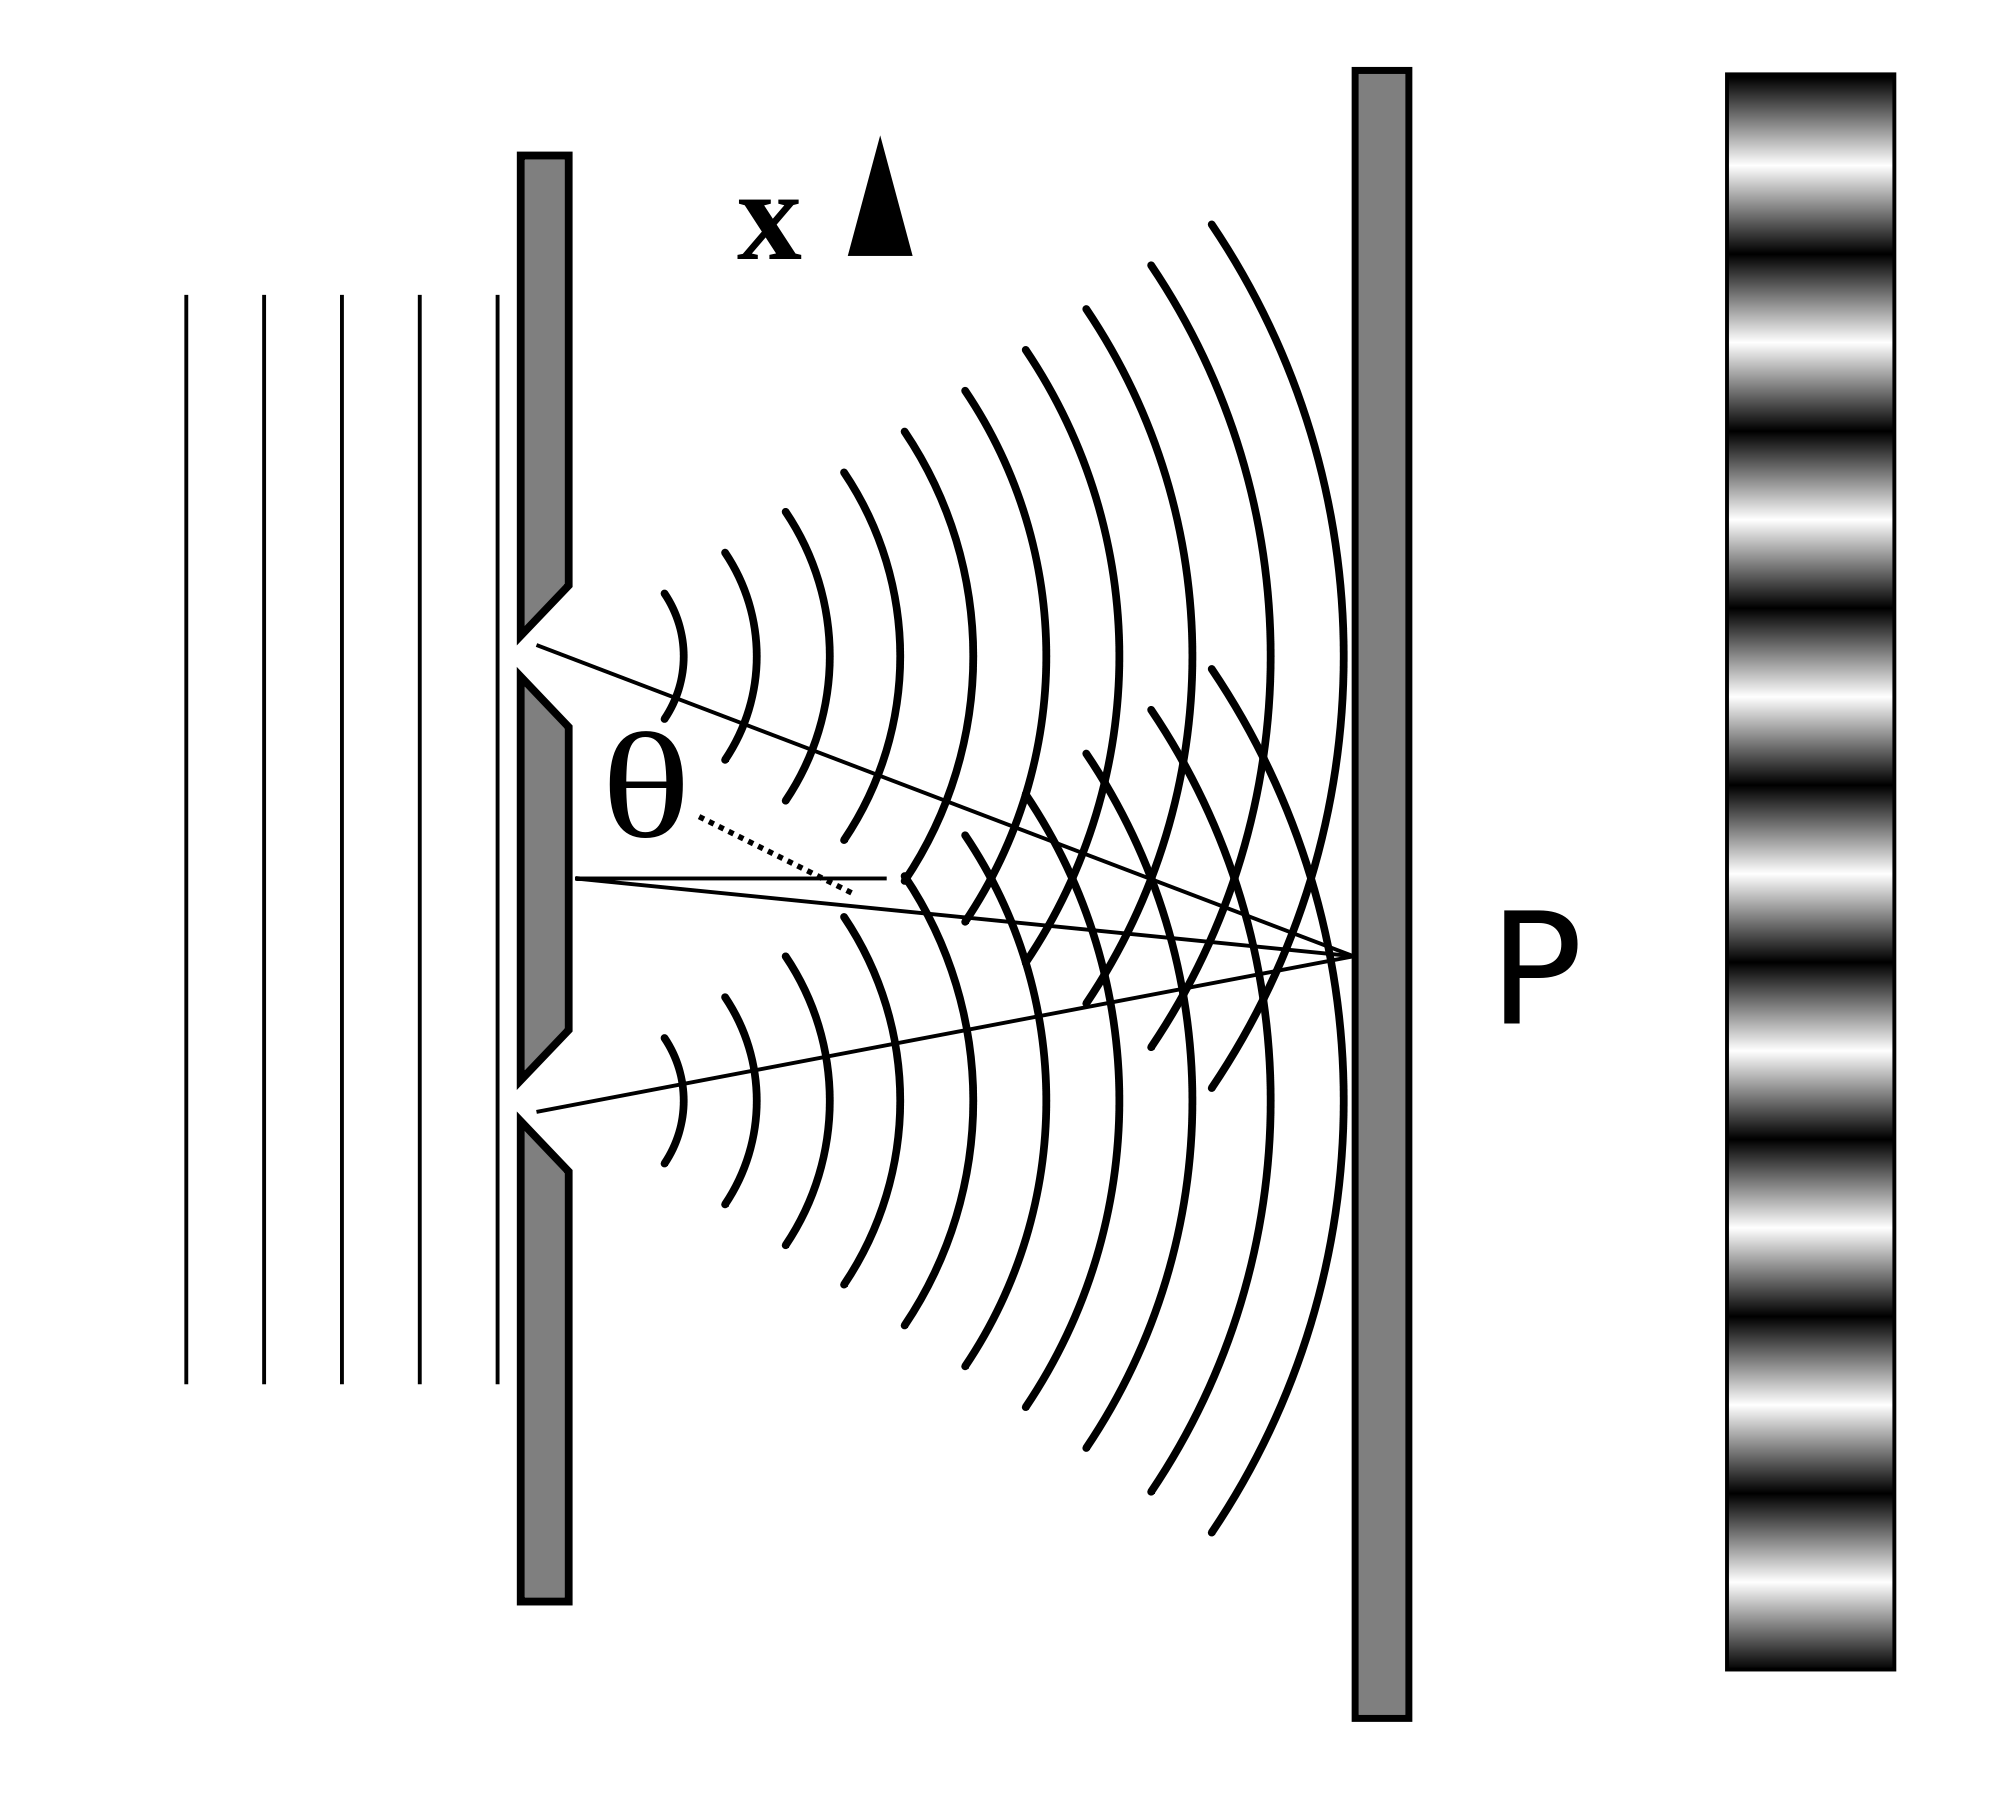
\includegraphics[width=0.4\textwidth]{doppelspalt.png}
    \caption{Doppelspaltexperiment \cite{TODO}}
    \label{fig:doppelspalt}
\end{figure}
% 2.2.3 Aufbau
Der Aufbau ist wie folgt (Abb. \ref{fig:doppelspalt}): Eine Lichtquelle (links, Wellenhochpunkte als Striche), welche auf eine Wand mit zwei Spalten zukommt. Daneben eine geschlossene Wand, auf der das Licht aufkommt (rechts).

% 2.2.4 Beobachtung
Die Lichtwellen werden am Doppelspalt in zwei Elementarwellen zerlegt. Diese überlappen und interferieren miteinander. Verfolgt man die Punkte konstruktiver Interferenz, gelangt man an die Maxima (Muster rechts, dunkel). Verfolgt man dagegen die Punkte destruktiver Interferenz, gelangt man an die Minima (Muster rechts, hell).
% 2.2.5 Schlussfolgerung
Die Maxima treten da auf, wo zwei Elementarwellen einen Gangunterschied eines Vielfachen von $\lambda$ haben, weil Konstruktive Interferenz auftritt (s. Formel \ref{eq:konstruktive_interferenz}). Die Minima treten da auf, wo der Gangunterschied um $\frac{\lambda}{2}$ verschoben ist (s. Formel \ref{eq:destruktive_interferenz}).


% 2.2._ Warum Grundlage?
% TODO